\subsection{Caso d'Uso: Aggiungi un Annuncio Immobiliare}

Per garantire un’esperienza utente ottimale, abbiamo progettato i mockup del caso d'uso \textit{Aggiungi un Annuncio Immobiliare} seguendo i principi della user experience (UX) e dell'usabilità. Il percorso utente è stato studiato attentamente per minimizzare il carico cognitivo e semplificare l’interazione, in linea con i modelli proposti da Nielsen e Norman \cite{nielsen1995,norman1988}.

\subsection*{Schermata Iniziale: Gestione Annunci Immobiliari}
L’azione di aggiungere un nuovo annuncio parte dalla schermata di Gestione Annunci Immobiliari, dove l’utente trova:
\begin{itemize}
    \item \textbf{Una lista degli immobili a lui associati}, che consente una rapida contestualizzazione.
    \item \textbf{Un pulsante unico ed evidente}, etichettato “Aggiungi Annuncio Immobiliare”, che centralizza l’azione primaria.
\end{itemize}

\subsection*{Flusso di Navigazione e Segmentazione del Form}
Al click del pulsante, l’utente viene indirizzato a una schermata dedicata alla compilazione di un form articolato in più step. Questa segmentazione si basa sul principio del \textbf{chunking dell’informazione} \cite{miller1956}, riducendo il carico di memoria e rendendo il processo meno gravoso. In particolare:
\begin{itemize}
    \item \textbf{Step 1:} Richiede le informazioni basilari, quali il titolo, il tipo di contratto e il tipo di immobile.
    \item \textbf{Step 2 e successivi:} Raccolgono i dati principali e le caratteristiche secondarie dell’immobile, organizzati in modo logico e intuitivo.
\end{itemize}

\subsection*{Navigazione Sticky e Accessibilità degli Step}
I pulsanti di navigazione, posizionati in alto con comportamento \textit{sticky}, consentono all’utente di passare agevolmente da uno step all’altro, anche in presenza di schermate particolarmente lunghe. Tale scelta:
\begin{itemize}
    \item Riduce il tempo necessario per individuare i controlli di navigazione.
    \item Favorisce un’interazione continua e fluida, in linea con i principi di design centrato sull’utente e le best practice in ambito HCI (Human-Computer Interaction) \cite{shneiderman2004}.
\end{itemize}

\subsection*{Integrazione della Mappa Interattiva}
Per quanto riguarda l’inserimento dell’indirizzo:
\begin{itemize}
    \item \textbf{La mappa interattiva} permette di visualizzare immediatamente la posizione indicata, offrendo un feedback visivo diretto.
    \item L’utente ha la possibilità di regolare la posizione direttamente sulla mappa, migliorando la precisione del dato inserito \cite{wickens2008}.
\end{itemize}

\subsection*{Gestione delle Immagini e Feedback Visivo}
La sezione dedicata alle immagini è progettata per:
\begin{itemize}
    \item \textbf{Consentire l’aggiunta di foto} tramite pulsante dedicato o drag and drop, facilitando l’upload in maniera intuitiva.
    \item \textbf{Permettere l’inserimento di una descrizione} per ogni immagine, migliorando la contestualizzazione visiva dell’annuncio \cite{pieters2004}.
\end{itemize}

\subsection*{Anteprima e Conferma Finale}
Infine, viene presentato uno schema riepilogativo che funge da anteprima dell’annuncio così come apparirà agli utenti finali. Una volta verificata la correttezza dei dati:
\begin{itemize}
    \item L’utente può cliccare il pulsante \textbf{“Pubblica”}, che innesca un processo di caricamento e validazione.
    \item Al termine del processo, viene mostrato un messaggio di conferma che attesta il successo dell’operazione, riducendo l’ansia da incertezza e rafforzando la fiducia nel sistema \cite{nielsen1995}.
\end{itemize}

\newpage

\begin{figure}[ht]
    \centering
    \begin{tikzpicture}[node distance=1.5cm and 1cm, auto]
        % Nodo per immagine 1 con didascalia sotto
        \node (img1) {
            \begin{tabular}{c}
                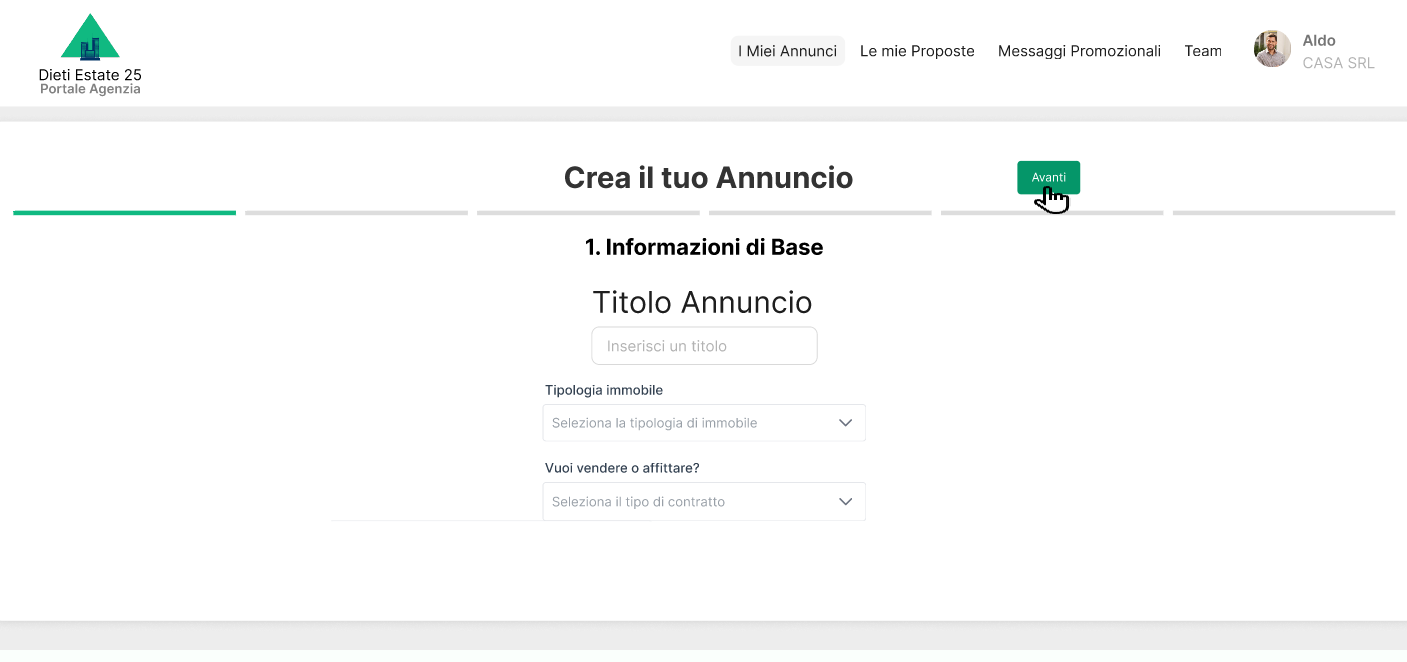
\includegraphics[width=0.7\textwidth]{Immagini/Mockup/aggiungi annuncio/scenario principale/step1.png} \\
                Cockburn: step 3
            \end{tabular}
        };
        
        % Nodo per immagine 2 con didascalia sotto, posizionato a destra di img1
        \node (img2) [below=of img1] {
            \begin{tabular}{c}
                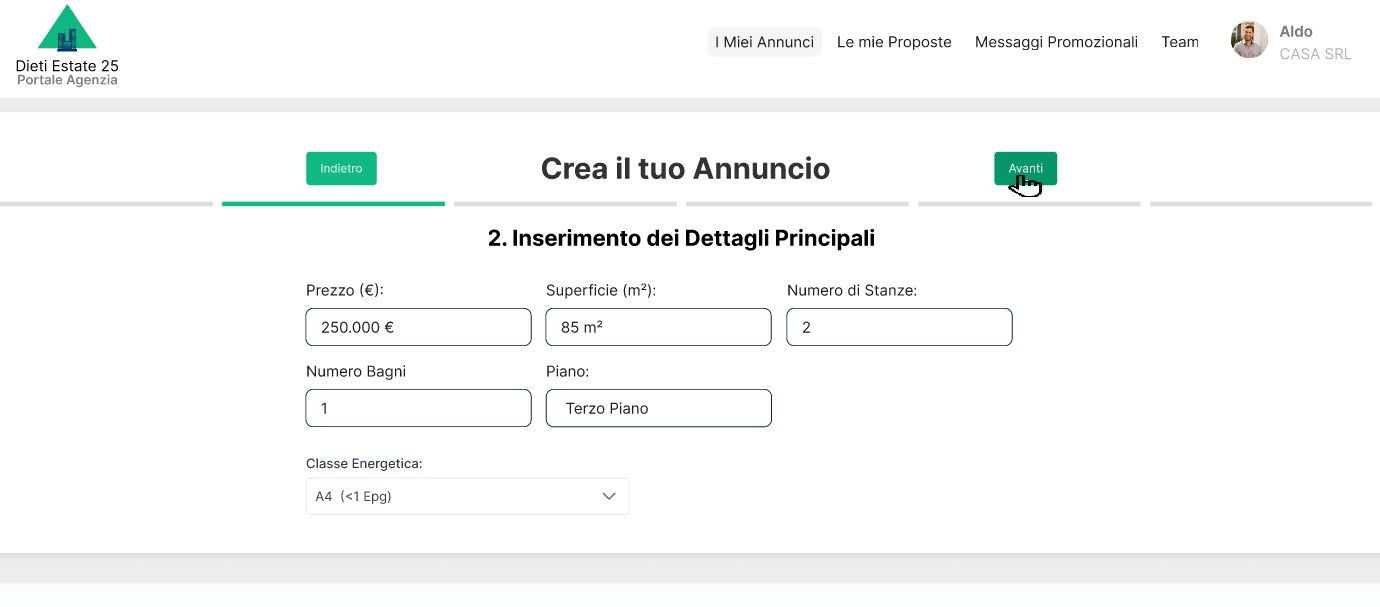
\includegraphics[width=0.7\textwidth]{Immagini/Mockup/aggiungi annuncio/scenario principale/step2.png} \\
                Cockburn: step4/5
            \end{tabular}
        };
        
        % Nodo per immagine 3 con didascalia sotto, posizionato sotto img2
        \node (img3) [below=of img2] {
            \begin{tabular}{c}
                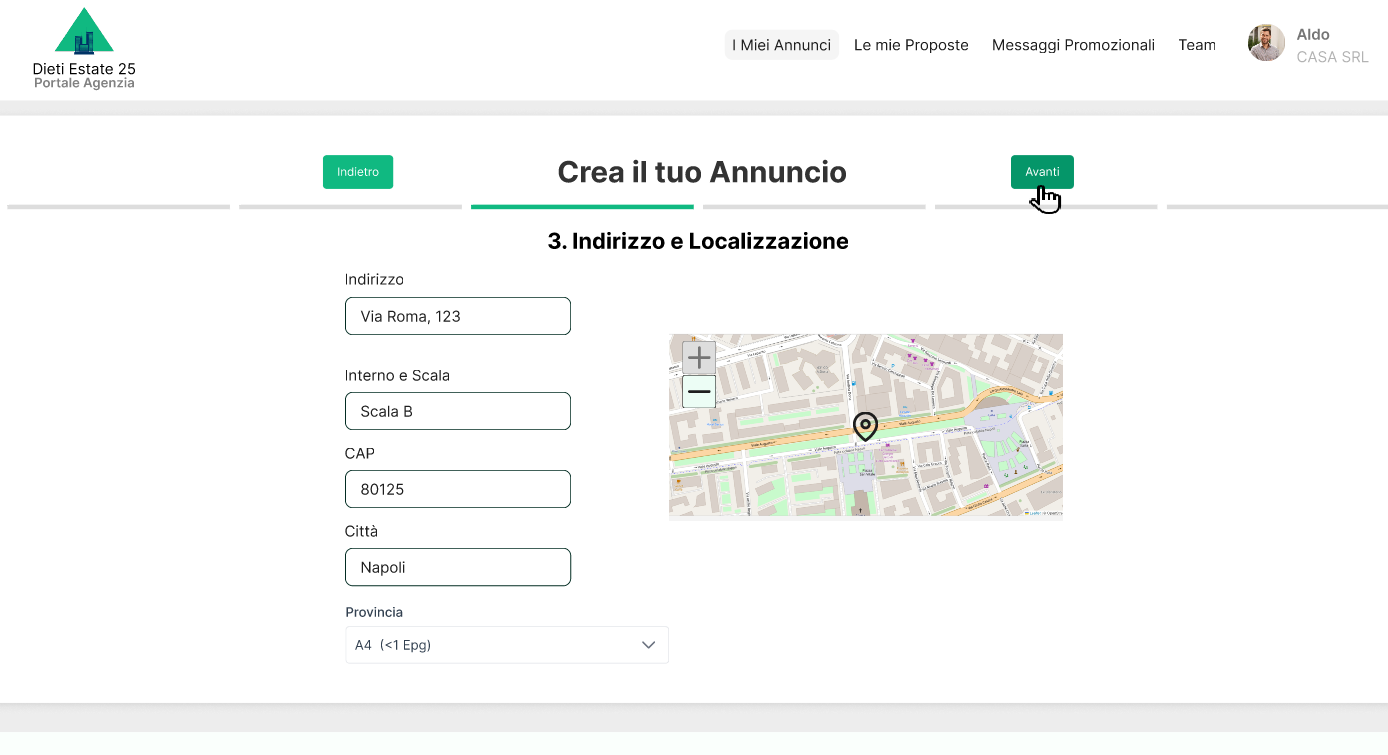
\includegraphics[width=0.7\textwidth]{Immagini/Mockup/aggiungi annuncio/scenario principale/step3.png} \\
                Cockburn: step 4/5
            \end{tabular}
        };
        
        % Disegna le frecce
        \draw[->, thick] (img1) -- (img2);
        \draw[->, thick] (img2) -- (img3);
      
    \end{tikzpicture}
    \caption{Mockup: scenario principale della tabella di Cockburn del caso d'uso nuovo annuncio.}
    \label{fig:mockup_scenario_principale_parte1_aggiungi_annuncio}
\end{figure}

\newpage



\begin{figure}[ht]
    \centering
    \begin{tikzpicture}[node distance=1.5cm and 1cm, auto]
        % Nodo per immagine 1 con didascalia sotto
        \node (img1) {
            \begin{tabular}{c}
                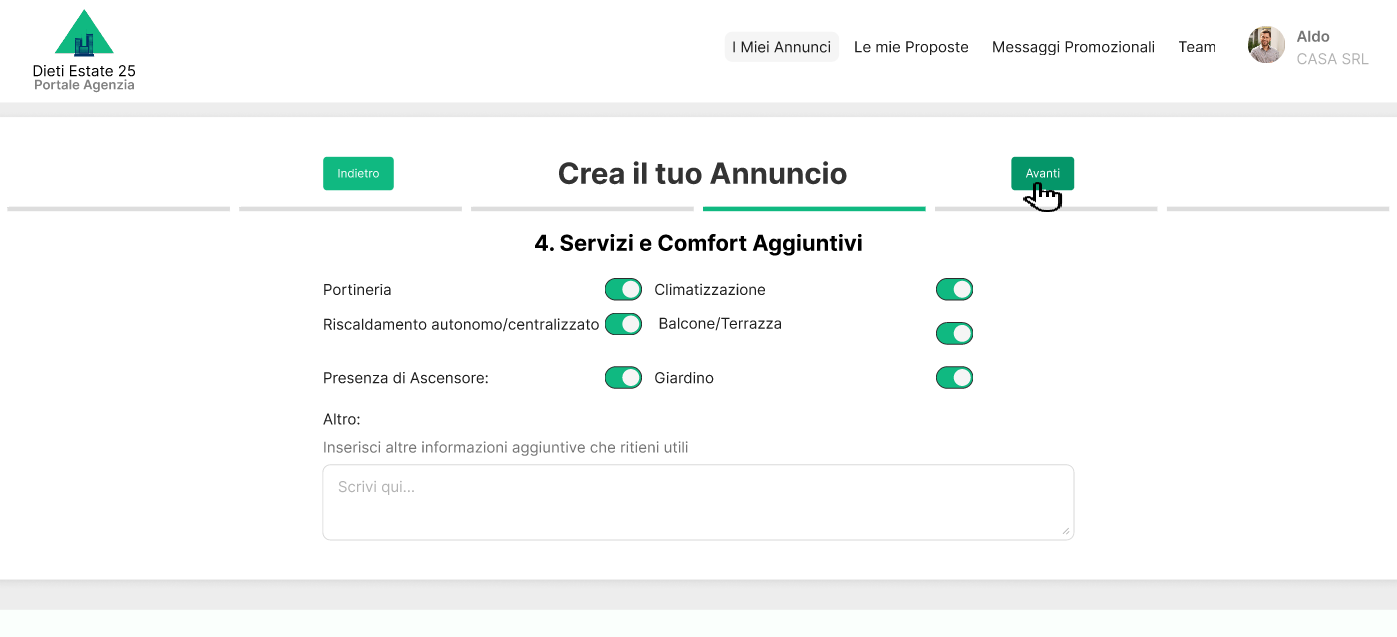
\includegraphics[width=\textwidth,keepaspectratio]{Immagini/Mockup/aggiungi annuncio/scenario principale/step4.png} \\
                Cockburn: step 4/5
            \end{tabular}
        };
        
        % Nodo per immagine 2 con didascalia sotto, posizionato a destra di img1
        \node (img2) [below=of img1] {
            \begin{tabular}{c}
                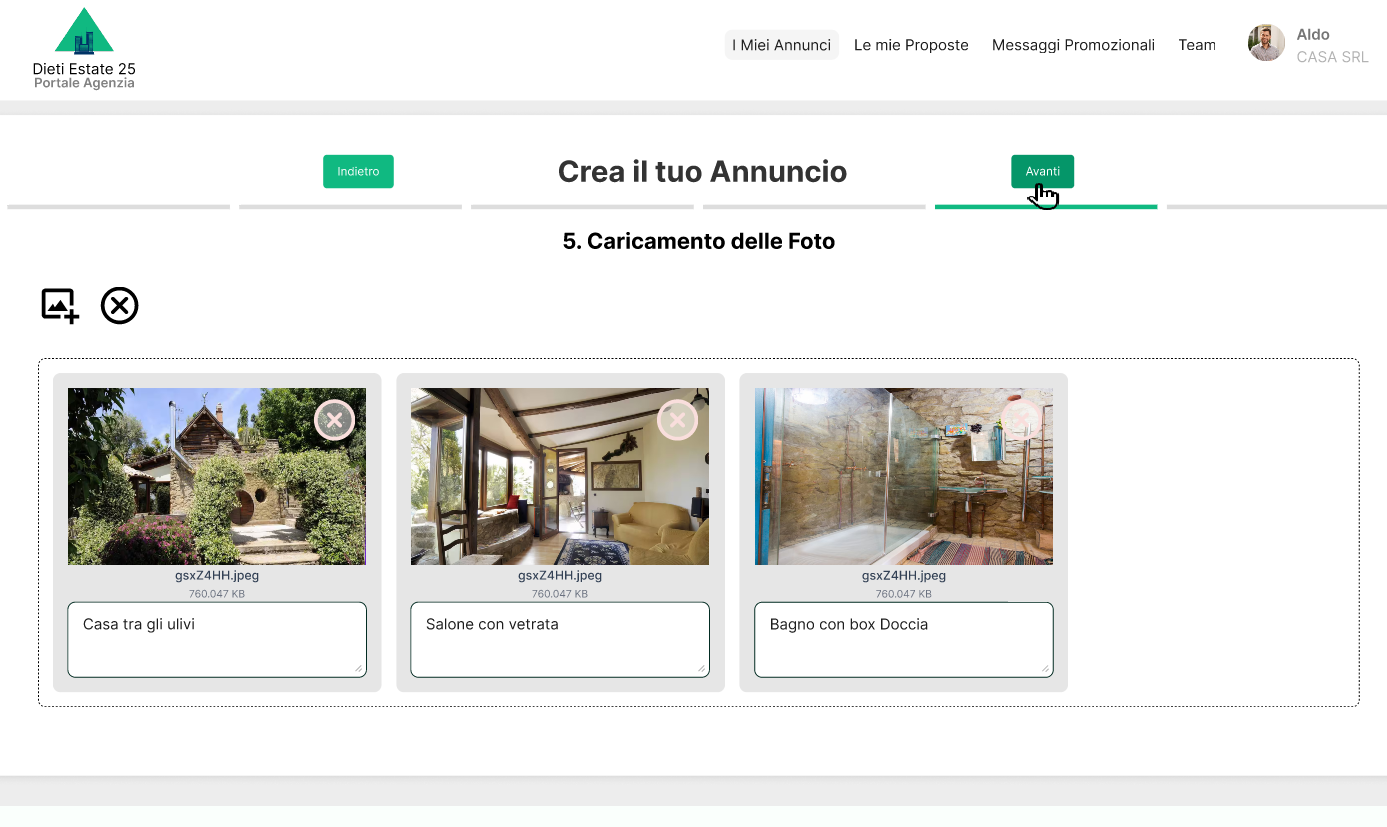
\includegraphics[width=\textwidth,keepaspectratio]{Immagini/Mockup/aggiungi annuncio/scenario principale/step5.png} \\
                Cockburn: step 6
            \end{tabular}
        };
        
        % Disegna le frecce
        \draw[->, thick] (img1) -- (img2);
      
    \end{tikzpicture}
    \caption{Mockup: scenario principale della tabella di Cockburn del caso d'uso nuovo annuncio.}
    \label{fig:tikz_flow}
\end{figure}

\newpage

\input{Requisiti Del Software/Analisi dei Requisiti/Mockup/aggiungi annuncio/scenario principale Parte III}



\clearpage
\newpage

\subsubsection{Estensione A: Disattivazione Notifiche dalla Visualizzazione di una Notifica}

Per offrire un maggiore controllo sulla gestione delle notifiche senza interrompere l’esperienza utente, il sistema permette di disattivare una categoria direttamente dalla visualizzazione di una notifica specifica. Questa variante è progettata per garantire una modifica consapevole delle preferenze, evitando azioni impulsive che potrebbero compromettere la ricezione di informazioni rilevanti.

\vspace{0.5cm}
\subsubsection{Interfaccia e Comportamento del Bottone}
Alla fine del testo di ogni notifica, se la relativa categoria è attiva, è presente un pulsante neutro con la dicitura “Disattiva notifiche”. Accanto al pulsante, un testo in grigio informa l’utente della funzione del pulsante, evitando ambiguità. L’utilizzo di colori non accesi e di un design discreto segue il principio della \textbf{gerarchia visiva} \cite{pieters2004}, scoraggiando azioni impulsive che potrebbero portare alla perdita involontaria di notifiche future.

\vspace{0.5cm}
\subsubsection{Modifica dello Stato e Feedback Visivo}
Quando l’utente clicca sul pulsante, il testo del pulsante cambia colore, diventando rosso, e il messaggio a fianco si aggiorna per sottolineare che la categoria di notifiche è stata disattivata. Questo utilizza il principio della \textbf{salienza visiva} \cite{nielsen1995}, enfatizzando il cambiamento e rendendo immediatamente chiara la conseguenza dell’azione.

\vspace{0.5cm}
\subsubsection{Incentivo alla Riattivazione}
Una volta disattivata una categoria tramite questa modalità, viene visualizzato un secondo pulsante con una call-to-action mirata per incentivare la riattivazione delle notifiche. Il design e il posizionamento del pulsante sfruttano il \textbf{principio dell’affordance} \cite{norman1988}, rendendo chiaro che l’utente ha la possibilità di tornare indietro sulla sua decisione in modo semplice e immediato.
\newline
Questa estensione si integra perfettamente con il modello generale di gestione delle notifiche, garantendo un’interazione fluida e coerente con le esigenze dell’utente. Nel caso in cui l’utente scelga di riattivare la categoria delle notifiche direttamente da una notifica, si passa all’\textbf{Estensione F}, che approfondisce questa modalità di gestione a partire dalle notifiche disattivate.
\begin{figure}[ht]
    \centering
    \begin{tikzpicture}[node distance=1.5cm and 1cm, auto]
        % Nodo per immagine 1 con didascalia sotto
        \node (img1) {
            \begin{tabular}{c}
                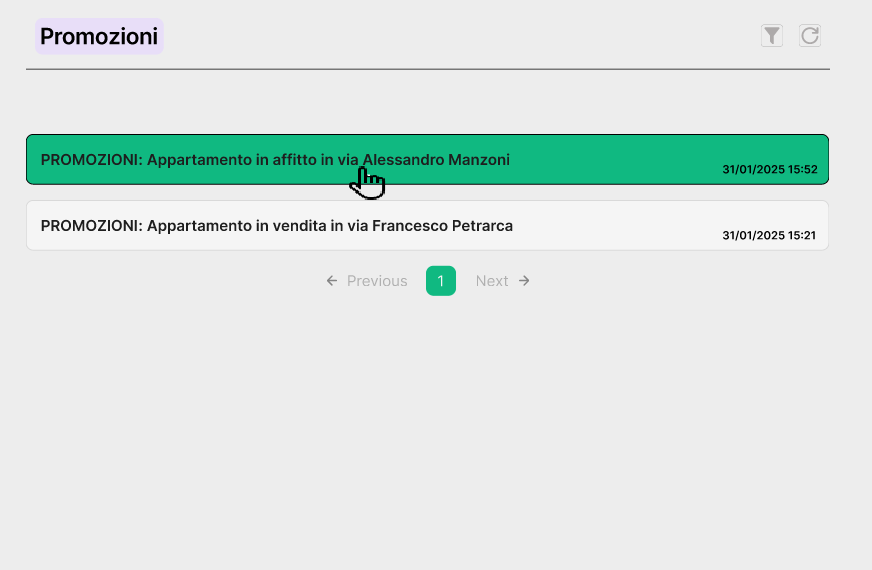
\includegraphics[width=0.4\textwidth]{Immagini/Mockup/notifiche/estensione A/clickNotifica.png} \\
                Cockburn: Extension A.2/A.3
            \end{tabular}
        };
        
        % Nodo per immagine 2 con didascalia sotto, posizionato a destra di img1
        \node (img2) [below=of img1] {
            \begin{tabular}{c}
                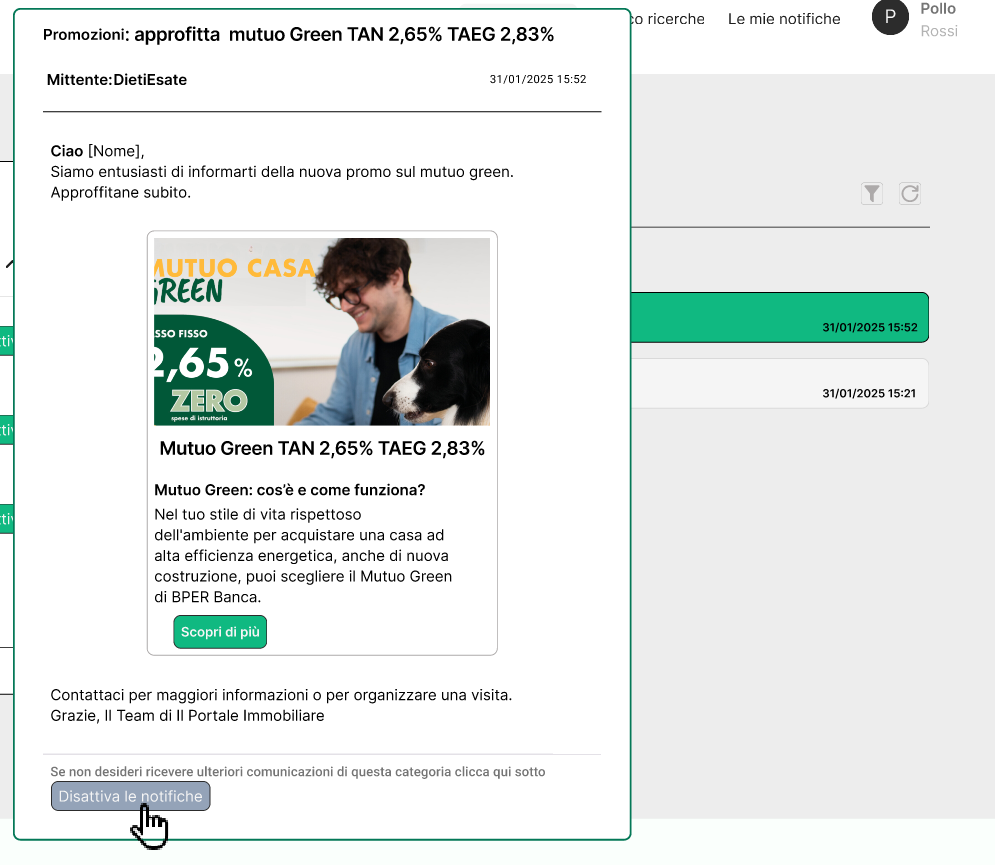
\includegraphics[width=0.4\textwidth]{Immagini/Mockup/notifiche/estensione A/clickDisattiva.png} \\
                Cockburn: Extension A.4
            \end{tabular}
        };
        
        % Nodo per immagine 3 con didascalia sotto, posizionato sotto img2
        \node (img3) [below=of img2] {
            \begin{tabular}{c}
                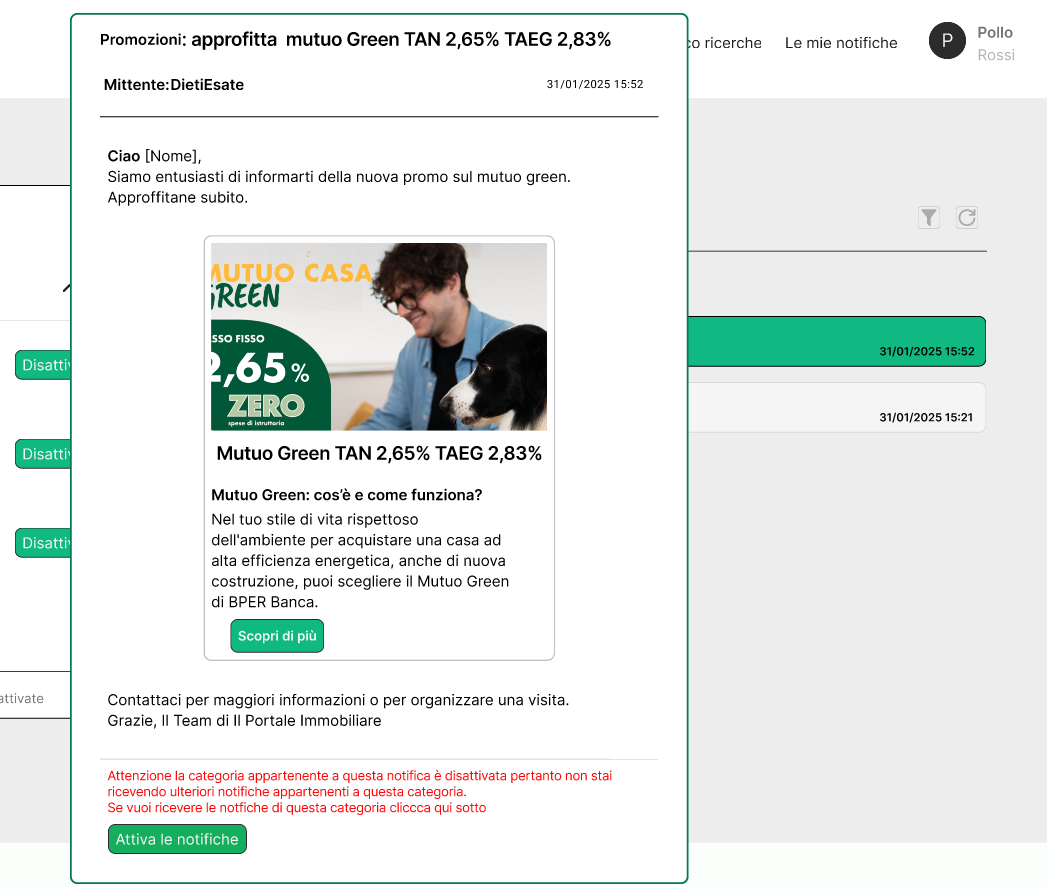
\includegraphics[width=0.4\textwidth]{Immagini/Mockup/notifiche/estensione A/disattivato.png} \\
                Cockburn: extension A.5
            \end{tabular}
        };
        
        % Disegna le frecce
        \draw[->, thick] (img1) -- (img2);
        \draw[->, thick] (img2) -- (img3);
      
    \end{tikzpicture}
    \caption{Mockup: estensione A della tabella di Cockburn del caso d'uso disattiva/attiva categoria notifica}
    \label{fig:mockup_estensione_A_disattiva_notifiche}
\end{figure}

\newpage



\clearpage
\newpage
\subsubsection{Estensione B: Ripristino di un Annuncio Precedente}
Se l’utente sceglie di \textbf{ripristinare l’annuncio precedente}, il sistema avvia un processo di caricamento per fornire un feedback visivo sulla ripresa dei dati. Sebbene i dati siano salvati localmente e il recupero sia immediato, un \textbf{indicatore di caricamento fittizio} viene mostrato per alcuni secondi prima di caricare la schermata.

Questa soluzione è basata sul principio della \textbf{coerenza con le aspettative dell’utente} \cite{shneiderman2004}. In un contesto digitale, un ripristino istantaneo potrebbe apparire innaturale e creare confusione. L’indicatore di caricamento:
\begin{itemize}
    \item Rafforza la percezione di un processo in corso, migliorando la trasparenza dell’operazione.
    \item Evita che l’utente si domandi se il recupero sia realmente avvenuto o se ci siano stati problemi tecnici.
    \item Contribuisce a una transizione più fluida tra stati dell’interfaccia.
\end{itemize}

Una volta completato il caricamento, il sistema presenta l’interfaccia con i dati precedentemente salvati, consentendo all’utente di riprendere il processo da dove era stato interrotto.


\begin{figure}[ht]
    \centering
    \begin{tikzpicture}[node distance=1.5cm and 1cm, auto]
        % Nodo per immagine 1 con didascalia sotto
        \node (img1) {
            \begin{tabular}{c}
                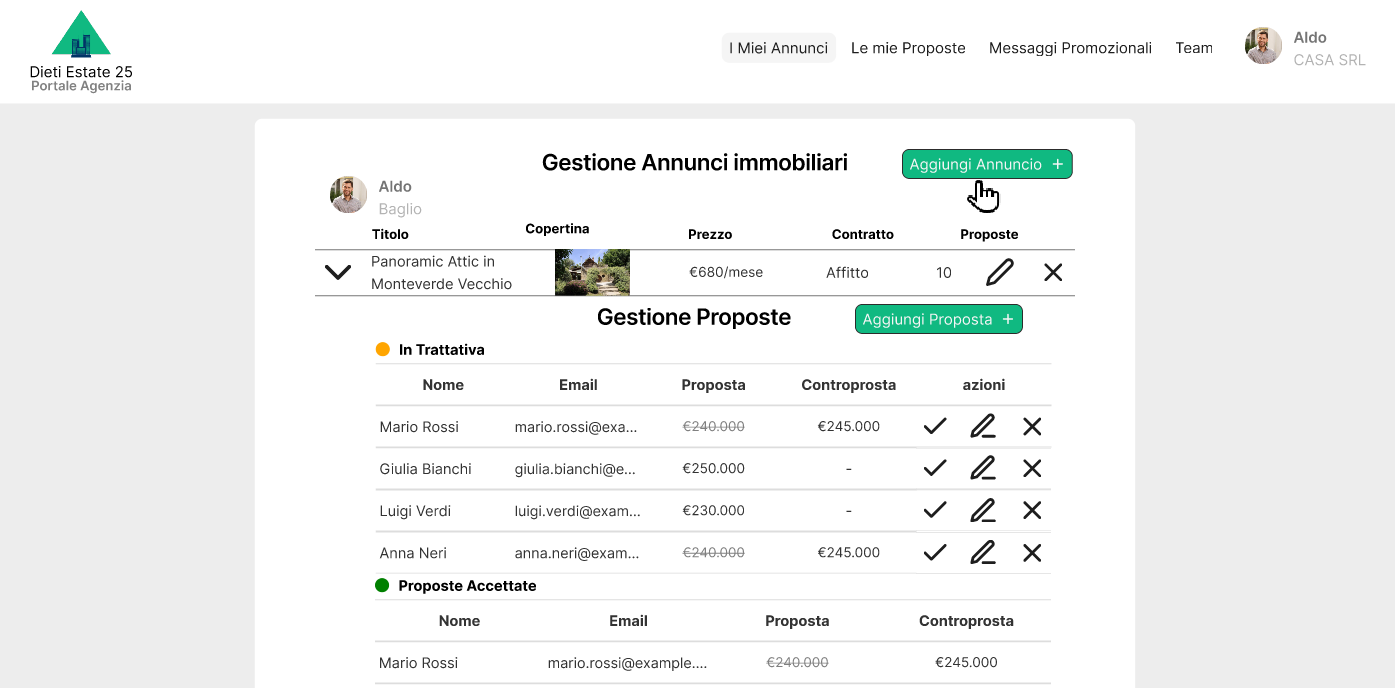
\includegraphics[width=0.7\textwidth]{Immagini/Mockup/aggiungi annuncio/estensione B/step1.png} \\
                click nuovo annuncio
            \end{tabular}
        };
        
        % Nodo per immagine 2 con didascalia sotto, posizionato a destra di img1
        \node (img2) [below=of img1] {
            \begin{tabular}{c}
                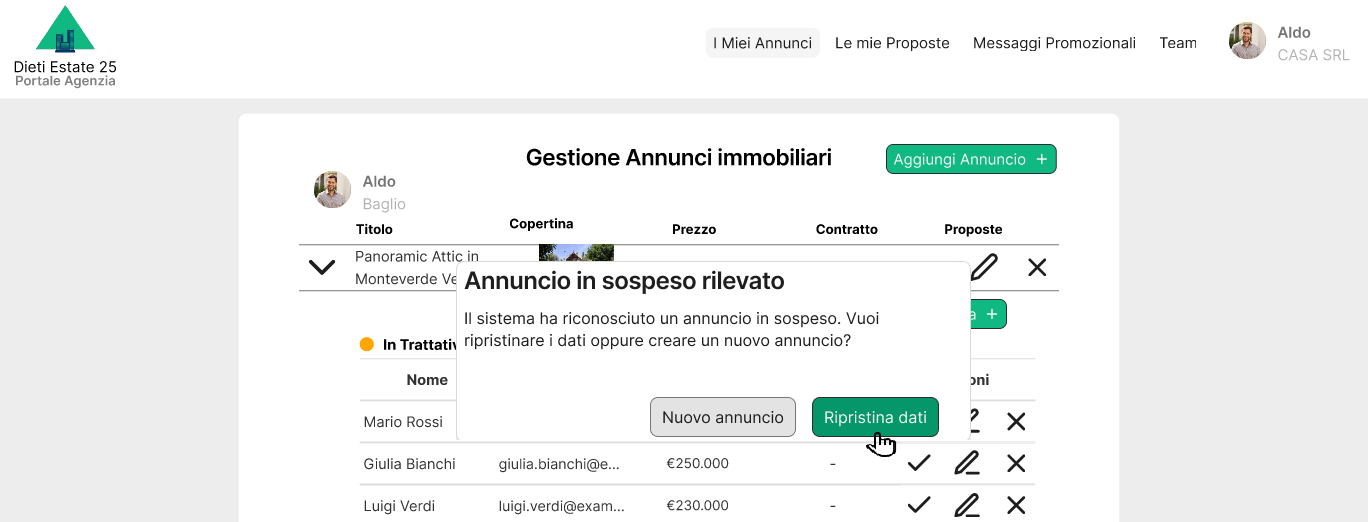
\includegraphics[width=0.7\textwidth]{Immagini/Mockup/aggiungi annuncio/estensione B/step2.png} \\
                Cockburn: extension B.2/B.3/B.4
            \end{tabular}
        };
        
        % Nodo per immagine 3 con didascalia sotto, posizionato sotto img2
        \node (img3) [below=of img2] {
            \begin{tabular}{c}
                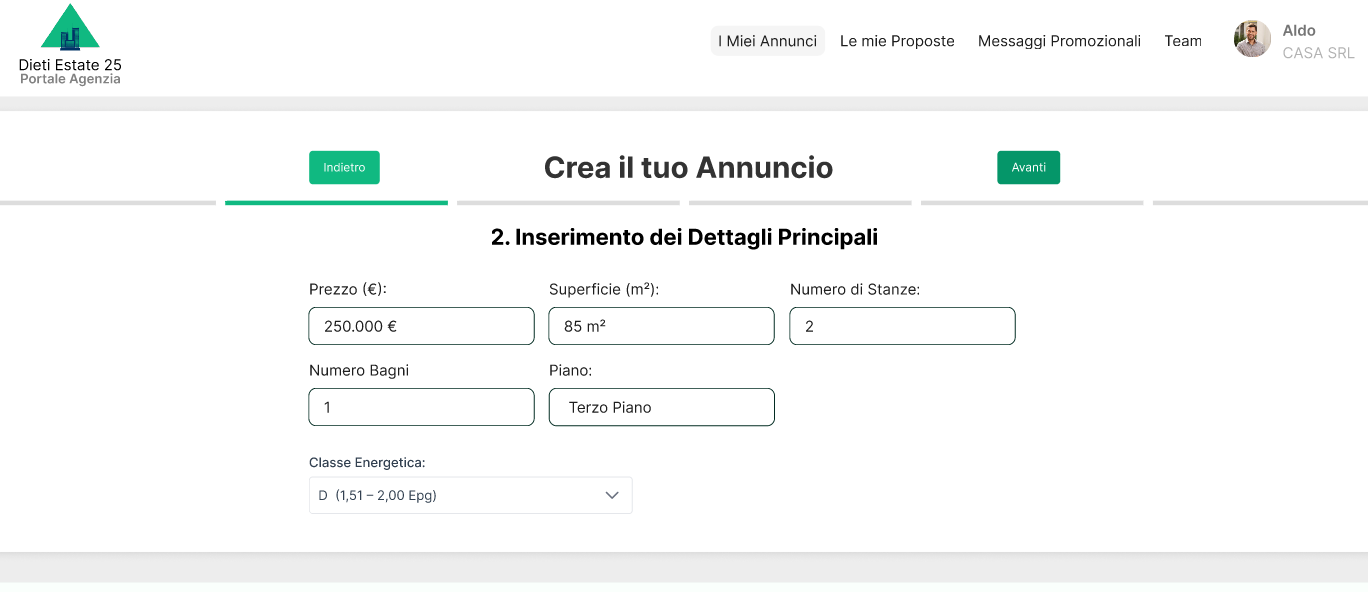
\includegraphics[width=0.7\textwidth]{Immagini/Mockup/aggiungi annuncio/estensione B/step3.png} \\
                Cockburn: extension B.5
            \end{tabular}
        };
        
        % Disegna le frecce
        \draw[->, thick] (img1) -- (img2);
        \draw[->, thick] (img2) -- (img3);
      
    \end{tikzpicture}
    \caption{Mockup: estensione B della tabella di Cockburn del caso d'uso nuovo annuncio}
    \label{fig:mockup_estensione_B_aggiungi_annuncio}
\end{figure}

\newpage




\clearpage
\newpage
\subsubsection{Estensione C: Errore Durante la Pubblicazione dell'Annuncio}

Nel caso in cui si verifichi un errore durante la pubblicazione dell'annuncio immobiliare, viene mostrato un popup informativo che comunica all'utente il problema riscontrato. Questo popup ha il compito di rassicurare l'utente che i dati inseriti non andranno persi, in quanto vengono salvati localmente, e invita a riprovare più tardi.

\subsubsection{Gestione dell'Errore e Feedback Utente}
Il popup presenta i seguenti elementi chiave:
\begin{itemize}
    \item \textbf{Messaggio chiaro e rassicurante}: informa l'utente dell'errore senza tecnicismi, riducendo il senso di frustrazione.
    \item \textbf{Pulsante “Riprova”}: consente di tentare nuovamente la pubblicazione con un'animazione di caricamento, per segnalare che l'azione è in corso e mantenere un senso di controllo e progressione.
    \item \textbf{Pulsante “Monstra i Dettagli”}: offre la possibilità di visualizzare l'errore tecnico riscontrato. Questa funzione segue i principi di trasparenza e controllo dell'utente, utili sia per utenti avanzati che per eventuali tecnici di supporto che potrebbero risolvere il problema più rapidamente.
\end{itemize}

\subsubsection{Principi di Design Applicati}
L'implementazione di questa gestione degli errori si basa su diversi principi della UX e dell'usabilità:
\begin{itemize}
    \item \textbf{Visibilità dello stato del sistema} \cite{nielsen1995}: l'animazione di caricamento fornisce un'indicazione chiara che il sistema sta lavorando sulla richiesta dell'utente.
    \item \textbf{Prevenzione degli errori} \cite{nielsen1995}: il salvataggio locale dei dati riduce la possibilità di perdere informazioni a causa di un problema temporaneo.
    \item \textbf{Fornire informazioni utili per il recupero dall'errore} \cite{nielsen1995}: il messaggio di errore è accompagnato da suggerimenti su come procedere e un'opzione per visualizzare i dettagli tecnici, utile per il supporto tecnico.
\end{itemize}

Queste soluzioni mirano a mantenere un'esperienza utente fluida e priva di frustrazione, minimizzando il disagio derivante da problemi tecnici imprevisti.


\begin{figure}[ht]
    \centering
    \begin{tikzpicture}[node distance=1.5cm and 1cm, auto]
        % Nodo per immagine 1 con didascalia sotto
        \node (img1) {
            \begin{tabular}{c}
                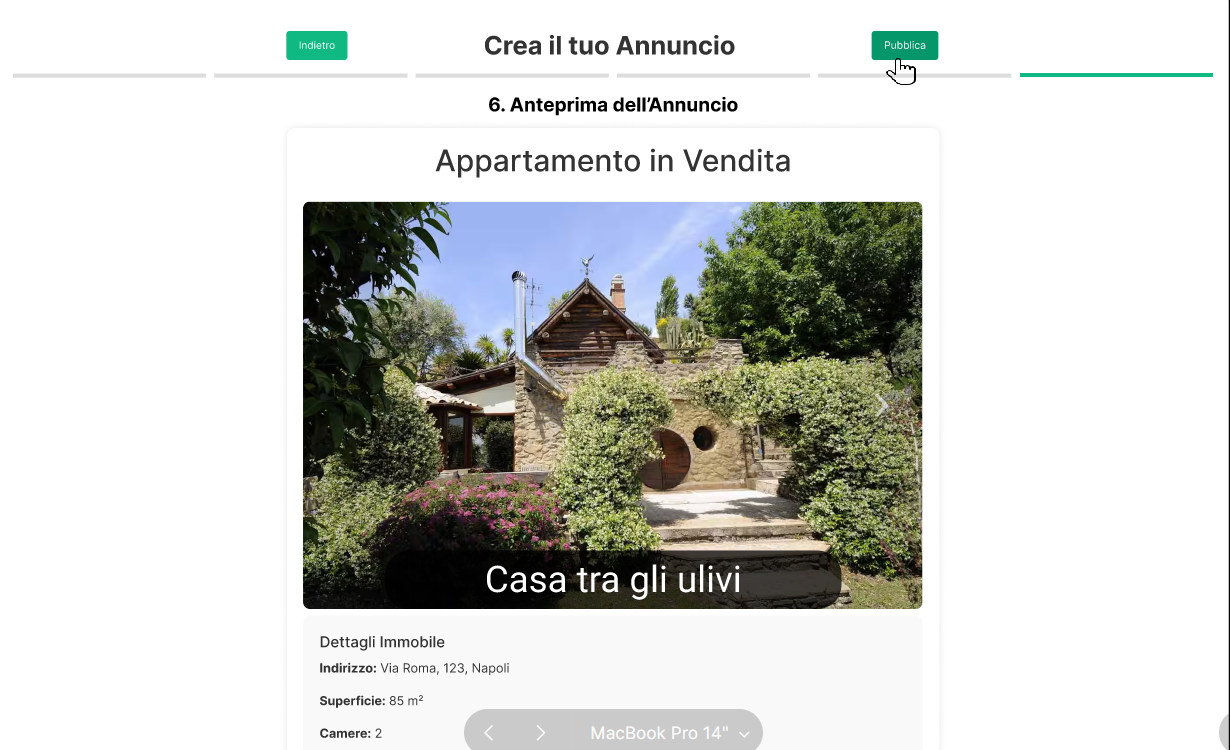
\includegraphics[width=0.7\textwidth]{Immagini/Mockup/aggiungi annuncio/estensione C/step1.png} \\
                click pubblica nuovo annuncio
            \end{tabular}
        };
        
        % Nodo per immagine 2 con didascalia sotto, posizionato a destra di img1
        \node (img2) [below=of img1] {
            \begin{tabular}{c}
                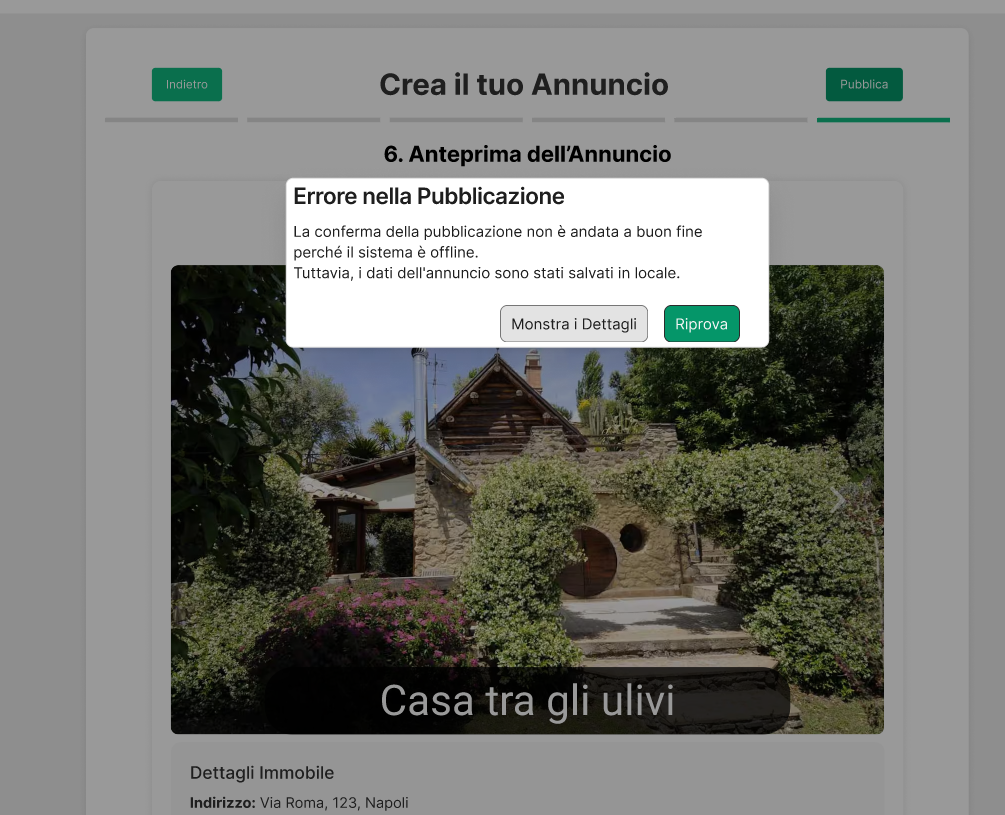
\includegraphics[width=\textwidth]{Immagini/Mockup/aggiungi annuncio/estensione C/step2.png} \\
                Cockburn: extension C.9/C.10
            \end{tabular}
        };
        
        
        % Disegna le frecce
        \draw[->, thick] (img1) -- (img2);
      
    \end{tikzpicture}
    \caption{Mockup: estensione C della tabella di Cockburn del caso d'uso nuovo annuncio}
    \label{fig:tikz_flow}
\end{figure}

\newpage



\clearpage
\newpage

\subsubsection{Estensione D: Modifica Rapida dello Stato delle Notifiche con Attivazione Immediata}

Questa variante rappresenta l’approccio duale dell’\textbf{Estensione C}, semplificando ulteriormente l’attivazione delle notifiche. L’obiettivo è ridurre i passaggi necessari per riattivare una categoria disattivata, mantenendo comunque un controllo chiaro sulla disattivazione.

\vspace{0.5cm}
\subsubsection{Interfaccia e Interazione}
Analogamente all’\textbf{Estensione C}, ogni categoria nella barra laterale dispone di un pulsante contestuale per modificarne lo stato. Il pulsante può assumere due stati:

\begin{itemize}
    \item \textbf{Attiva}, se la categoria è attualmente disabilitata.
    \item \textbf{Disattiva}, se la categoria è attualmente abilitata.
\end{itemize}

Le interazioni dell’utente variano a seconda dell’azione eseguita:

\begin{itemize}
    \item \textbf{Disattivazione di una categoria}:
    \begin{itemize}
        \item Al clic su \textbf{Disattiva}, appare un popup di conferma che informa l’utente sulle conseguenze della scelta, prevenendo azioni accidentali in linea con i principi di Nielsen \cite{nielsen1995}.
        \item Se confermata, la categoria viene spostata nella sezione delle notifiche disattivate tramite un’animazione di transizione.
        \item Il pulsante cambia stato, diventando \textbf{Attiva}, fornendo un feedback visivo chiaro sulla modifica.
    \end{itemize}
    
    \item \textbf{Attivazione di una categoria}:
    \begin{itemize}
        \item Al clic su \textbf{Attiva}, il sistema aggiorna immediatamente lo stato della notifica senza richiedere una conferma esplicita.
        \item La categoria viene spostata nella sezione delle notifiche attive con un’animazione fluida, applicando il principio della \textbf{gestalt della continuità} \cite{miller1956}.
        \item Il pulsante cambia stato in \textbf{Disattiva}, rendendo la modifica evidente e intuitiva.
    \end{itemize}
\end{itemize}

\subsubsection{Feedback Visivo e UX Design}
L’esperienza utente è ottimizzata tramite tecniche di design che garantiscono chiarezza e immediatezza:

\begin{itemize}
    \item \textbf{Popup di conferma per la disattivazione}: aiuta a prevenire errori e rende consapevole l’utente delle conseguenze della scelta \cite{nielsen1995}.
    \item \textbf{Animazione di transizione}: assicura una continuità visiva fluida nello spostamento delle categorie, migliorando la percezione del cambiamento \cite{miller1956}.
    \item \textbf{Aggiornamento immediato dello stato del pulsante}: il cambio di testo e colore riflette lo stato corrente della categoria, riducendo l’ambiguità e migliorando la prevedibilità dell’interazione.
\end{itemize}

Questa estensione semplifica l’attivazione delle notifiche, eliminando il passaggio della conferma e migliorando la fluidità dell’interazione, senza compromettere il controllo dell’utente sulla gestione delle proprie preferenze.

\begin{figure}[ht]
    \centering
    \begin{tikzpicture}[node distance=1.5cm and 1cm, auto]
        % Nodo per immagine 1 con didascalia sotto
        \node (img1) {
            \begin{tabular}{c}
                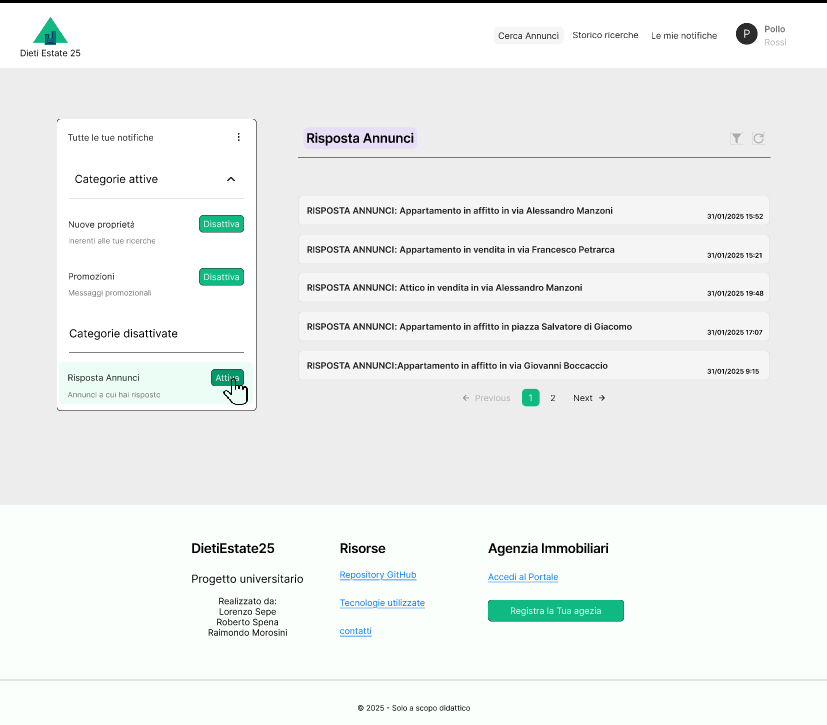
\includegraphics[width=0.6\textwidth]{Immagini/Mockup/notifiche/estensione D/clickAttiva.png} \\
                Cockburn: Extension D.2
            \end{tabular}
        };
        
        % Nodo per immagine 2 con didascalia sotto, posizionato a destra di img1
        \node (img2) [below=of img1] {
            \begin{tabular}{c}
                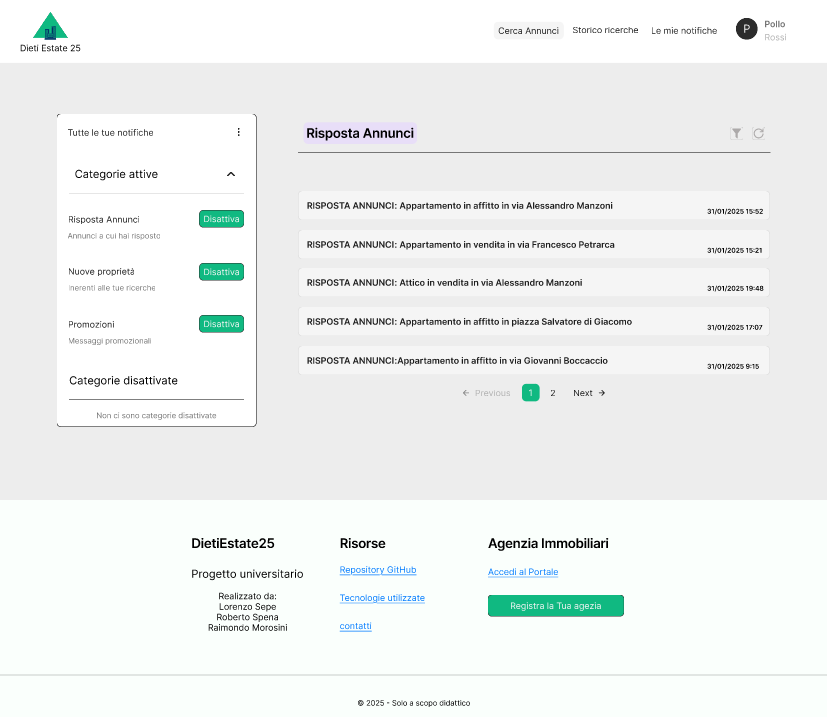
\includegraphics[width=0.6\textwidth]{Immagini/Mockup/notifiche/estensione D/attivato.png} \\
                Cockburn: step 8/9/10
            \end{tabular}
        };
        
        % Disegna le frecce
        \draw[->, thick] (img1) -- (img2);
      
    \end{tikzpicture}
    \caption{Mockup: estensione D della tabella di Cockburn del caso d'uso disattiva/attiva categoria notifica}
    \label{fig:mockup_estensione_D_disattiva_notifiche}
\end{figure}

\newpage

